\documentclass{beamer}
\usepackage{outlines}

\title{Warps}
\author{Mendocino College - Digital Image Manipulation with Photoshop}
\titlegraphic{\vspace{-10mm}
\includegraphics[width = .9\textwidth]{images/photoshop.jpg}} 
\date{\vspace{-5em}} 

\mode <presentation>
\usetheme{Warsaw}
\usecolortheme{default}

\setbeamerfont{footline}{size=\fontsize{5}{8}\selectfont}

\definecolor{darkred}{rgb}{20,0,0}
\definecolor{darkgreen}{RGB}{40,110,20}
\definecolor{darkpurple}{RGB}{30,0,30}
\definecolor{chardonnay}{RGB}{255, 255, 204}
\setbeamercolor*{palette primary}{fg=white, bg=darkgreen}

\setbeamersize{text margin left=0pt, text margin right=0pt}


\begin{document}
	{
		\setbeamertemplate{footline}{} 
		\setbeamertemplate{headline}{} 
		\begin{frame}
			\vspace{-35pt}
			\maketitle
		\end{frame}
	}
		
		
\section{Transform Warp}

\subsection{What it is and How to use it}		

	\begin{frame}
		\frametitle{What is Transform Warp?}
		\begin{outline}
			\1 The Warp command lets you drag control points to manipulate the shape of images, shapes, or paths, and so on. 
			\1 You can also warp using a shape in the Warp pop‑up menu in the options bar. 
			\1 Shapes in the Warp pop‑up menu are also malleable; you can drag their control points.
		\end{outline}
	\end{frame}

	\begin{frame}
	\frametitle{How to use Transform Warp}
	\begin{outline}
		\1 Select a layer 
		\2 (optional) select an area in the image with a selection tool.  
		\1 Choose Edit, in the menu bar
		\2 Click on Transform 
		\2 Select Warp 
		\1 Or Press Control + T (Win) / Cmd + T (Mac) 
		\2 Click the Switch Between Free Transform And Warp Modes button, in the options bar.
		\1 When you are finished, Press Enter (Windows) or Return (macOS), or click the Commit button in the options bar.
	\end{outline}
\end{frame}

\subsection{Example}		
	\begin{frame}
		\frametitle{Transform Warp Example}
		\begin{center}
			\includegraphics[width=1.0\textwidth]{images/Transform Warp example.png}
		\end{center}
	\end{frame}

\subsection{Options}		
	\begin{frame}
		\frametitle{Transform Warp Options}
		\begin{outline}
			\1 You can choose pre-made warp options.
			\1 Custom allows you to warp the image yourself by clicking and dragging anywere within the grid mesh.
		\end{outline}
	\begin{center}
	\includegraphics[width=0.75\textwidth]{images/transform warp options.png}
\end{center}
	\end{frame}

	\begin{frame}
	\frametitle{Transform Warp Options}
	\begin{outline}
		\1 To show or hide the warp mesh and control points, you can also choose View $\rightarrow$ Extras (from the menu bar).
		\1 To manipulate the shape, drag the control points, a segment of the bounding box or mesh, or an area within the mesh. 
		\2 When adjusting a curve, use the control point handles. 
		\2 This is similar to adjusting the handles in the curved segment of a vector graphic.
		\1 Click on a grid line to activate control points for editing the warp. 
		\2 Click on an anchor point (at the intersection of the grid lines) lets you edit the control points surrounding that anchor. 
		\2 Drag the control points to warp the image.
	\end{outline}
\end{frame}

\begin{frame}
	\frametitle{Transform Warp Options}
	\begin{outline}
		\1 To select multiple points, Shift+click on the anchor points or click-and-drag the pointer over the points while holding down the Shift key. 
		\2 A rectangle appears around the selected points if two or more points are selected. 
		\1 To deselect multiple points, Shift+click on the active anchor points or click-and-drag the pointer over the active points while holding down the Shift key. 
		\2 The rectangle surrounding the selected points automatically resizes as points are selected or deselected. 
		\1 To delete a selected grid line (control points along the line are visible), press Delete or choose Edit $\rightarrow$ Transform $\rightarrow$ Remove Warp Split. 
		\1 To delete both the horizontal and vertical grid lines passing through an anchor point, click the anchor point, then press Delete or choose Edit $\rightarrow$ Transform $\rightarrow$ Remove Warp Split.  
	\end{outline}
\end{frame}

\begin{frame}
	\frametitle{Transform Warp Options}
	\begin{outline}
		\1 To change the orientation of a warp style that you chose from the Warp menu, click the Change The Warp Orientation button in the options bar.
		\1 To change the reference point, click a square on the Reference point locator in the options bar.
		\1 To specify the amount of warp using numeric values, enter the values in the Bend (set bend), X (set horizontal distortion), and Y (set vertical distortion) text boxes in the options bar. 
		\2 You can’t enter numeric values if you have chosen None or Custom from the Warp Style pop‑up menu.
	\end{outline}
\end{frame}

\subsection{Resources}		
	\begin{frame}
		\frametitle{Additional Resources for the Transform Warp}
		\begin{outline}
			\1 Warp images, shapes, and paths
			\2 By:  Adobe
			\2 https://helpx.adobe.com/photoshop/using/warp-images-shapes-paths.html
			\1 how to use the Photoshop WARP tool to correct lens distortion without cropping your photo
			\2  By:  Steve Arnold
			\2 https://youtu.be/-coJI\_fIGIs
		\end{outline}
	\end{frame}


\section{Perspective Warp}

\subsection{What it is and How to use it}		

\begin{frame}
	\frametitle{What is Perspective Warp?}
	\begin{outline}
		\1 Sometimes, an object may look different in an image from how it appears in real life. 
		\2 This mismatch is due to perspective distortion. 
		\2 Images of the same object captured from different camera distances and angles of view exhibit different perspective distortion.
		\1 Photoshop lets you easily adjust perspective in images. 
		\1 This feature is particularly useful for images having straight lines and flat surfaces—for example, architectural images and images of buildings. 
		\1 You can also use this feature to composite objects having different perspectives in a single image.
	\end{outline}
\end{frame}

\begin{frame}
	\frametitle{How to use Perspective Warp - Define Planes}
	\begin{outline}
		\1 Before you adjust perspective, you must define the planes of the architecture in the image:
		\2 Open the image in Photoshop.
		\2 Choose Edit $\rightarrow$ Perspective Warp. (Review the onscreen tip and close it.)
		\2 Draw quads along the planes of the architecture in the image. 
		\3 While drawing the quads, try to keep their edges parallel to the straight lines in the architecture.
	\end{outline}
	\begin{center}
	\includegraphics[width=0.475\textwidth]{images/perspective warp 1.png}
\end{center}
\end{frame}

\begin{frame}
	\frametitle{How to use Perspective Warp - Manipulate Planes}
	\begin{outline}
		\1 Now you must manipulate the planes.
		\2 Switch to the Warp mode from the Layout mode.
		\2 Manipulate perspective in one of the available ways:
		\3 Move around the corners of the quads (pins) as appropriate.
		\2 Shift-click an individual edge of a quad to straighten it and keep it straight during further perspective manipulation. 
		\3 Such a straightened edge is highlighted in yellow in the Warp mode. 
		\3 You can manipulate the corners of the quads (pins) for finer control while adjusting perspective.
		\2 In the Warp mode, you can click the following icons for automatic perspective adjustment:
		\3 Automatically level near horizontal lines
		\3 Automatically straighten near vertical lines
		\3 Automatically straighten both vertically and horizontally
		\2 Once you're done adjusting the perspective, click the Commit Perspective Warp icon.
	\end{outline}
\end{frame}

\subsection{Example}	
\begin{frame}
	\frametitle{Perspective Warp Example}
	\begin{center}
		\includegraphics[width=1.0\textwidth]{images/perspective warp 2.png}
	\end{center}
\end{frame}
	
\begin{frame}
	\frametitle{Perspective Warp Example}
	\begin{center}
		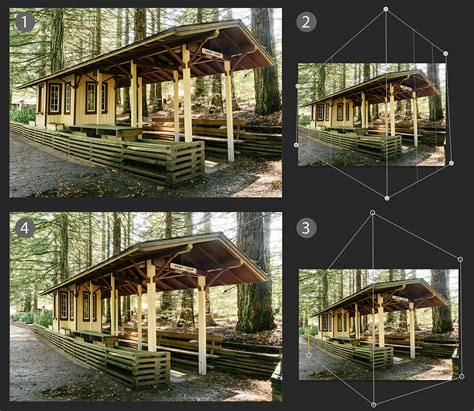
\includegraphics[width=0.7\textwidth]{images/Perspective Warp example.jpg}
	\end{center}
\end{frame}

\subsection{Options}		
\begin{frame}
	\frametitle{Perspective Warp Options}
	\begin{outline}
		\1 The following keyboard shortcuts make it easier to adjust perspective:
		\2 Arrow keys
		\3 Slightly move a corner of a quad (pin)
		\2 H
		\3 Hides the grid when you're working in the Warp mode
		\2 L
		\3 Switches to the Layout mode
		\2 W
		\3 Switches to the Warp mode
		\2 Enter key
		\3 In the Layout mode, switch to the Warp mode. 
		\3 In the Warp mode, commits the current changes.
		\2 Shift-click
		\3 (Warp Mode) Straightens an individual edge and keeps it straight. 
		\3 If you don't want to preserve the straightening of the edge, Shift-click it again.
		\2 Shift-(drag an edge)
		\3 (Layout mode) Constrains the shape of a plane while lengthening it
	\end{outline}
\end{frame}

\subsection{Resources}		
\begin{frame}
	\frametitle{Additional Resources for the Perspective Warp}
	\begin{outline}
		\1 Perspective Warp
		\2  By:  Adobe
		\2 https://helpx.adobe.com/photoshop/using/perspective-warp.html
		\1 How to Change The Perspective of ANYTHING In Photoshop - Perspective Warp Guide
		\2  By:  Photoshop Training Channel
		\2 https://youtu.be/vPMEWHKVffc
	\end{outline}
\end{frame}

\section{Puppet Warp}

\subsection{What it is and How to use it}		

\begin{frame}
	\frametitle{Puppet Warp}
	\begin{outline}
		\1 Puppet Warp provides a visual mesh that lets you drastically distort specific image areas, while leaving other areas intact. 
		\1 You can distort the image by dragging over the pins that you create over the mesh.
		\1 Applications range from subtle image retouching (such as shaping hair) to total transformations (such as repositioning arms or legs).
	\end{outline}
\end{frame}

	\begin{frame}
	\frametitle{How to use Puppet Warp}
	\begin{outline}
		\1 First, Convert the image to a smart object:
		\2 Select the layer
		\2 Then right-click
		\2 Select "Convert to Smart Object"
		\1 Choose Edit $\rightarrow$ Puppet Warp. 
		\1 In the image window, click to add pins to areas you want to transform and areas you want to anchor in place.
		\1 Drag the pins to warp the mesh.
		\1 To rotate the mesh a fixed number of degrees, press Alt (Windows) or Option (Mac OS), and position the cursor near to, but not over the pins. 
		\2 When a circle appears, drag to visually rotate the mesh.
		\2 To rotate the mesh automatically based on the selected Mode option, choose Auto from the Rotate menu in the options bar.  
		\1 When your transformation is complete, press Enter or Return.
	\end{outline}
\end{frame}

\subsection{Example}		
\begin{frame}
	\frametitle{Puppet Warp Example}
	\begin{center}
		\includegraphics[width=1.0\textwidth]{images/puppet warp example.jpg}
	\end{center}
\end{frame}

\subsection{Options}		
\begin{frame}
	\frametitle{Puppet Warp Options}
	\begin{outline}
		\1 Mode - 
		\2 Determines the stretchiness of the mesh.
		\2 Distort is for a highly elastic mesh, good for warping wide-angle images or texture maps.
		\2 Rigid is the exact opposite effect, by having less elasticity than the Normal.
		\1 Density - 
		\2 Determines the spacing of mesh points. Having fewer points gives you less precise control. 
		\2 Having more points increases precision, but requires more processing time.
		\1 Expansion - 
		\2 Expands or contracts the edge of the mesh.
		\1 Show Mesh - 
		\2 Deselect to show only adjustment pins, making your adjustments easier to see.
	\end{outline}
\end{frame}

\begin{frame}
	\frametitle{Puppet Warp Keyboard Shortcuts}
	\begin{outline}
		\1 Ctrl + A (Mac: Cmd + A) – Select all pins.
		\1 Ctrl + D (Mac: Cmd + D) – Deselect all pins.
		\1 Shift-Click on any pins to select multiple pins.
		\1 Hold down the H key to hide pins. Release to bring back the pins.
		\1 Alt-Click (Mac: Option-Click) on a Pin to Delete it.
		\1 Hold Alt (Mac: Option) near to, but not over a pin to reveal a circle that allows you to rotate the pin.
		\1 Press Delete to remove selected pins.
		\1 Press the Esc key to cancel distortions.
	\end{outline}
\end{frame}

\subsection{Resources}		
\begin{frame}
	\frametitle{Additional Resources for the Puppet Warp}
	\begin{outline}
		\1 How To Use Puppet Warp in Photoshop – Puppet Warp Guide
		\2  By:  Photoshop Training Channel
		\2 https://photoshoptrainingchannel.com/puppet-warp-in-photoshop/
		\1 Photoshop Puppet Warp 101: Everything You Wanted To Know
		\2  By:  Photoshop Training Channel
		\2 https://youtu.be/xRGt7byhS50
	\end{outline}
\end{frame}
	
\end{document}